\documentclass[12pt, a4paper]{article}


% A pretty common set of packages
\usepackage[margin=2.5cm]{geometry}
\usepackage[T1]{fontenc}
\usepackage{graphicx}
\usepackage{amssymb}
\usepackage{amsmath}
\usepackage{bm}
\usepackage{color}
\usepackage{float}
\usepackage{bm}
\usepackage{physics}
\usepackage{subcaption}

\begin{document}

\section{Theory}
\subsection{Question 1}
Based on the assumption that there is no noise or error in the control system,
predict the next pose $p_{t+1}$ as a nonlinear function of the current pose $p_t$ and
the control inputs $d_t$ and $\alpha_t$. (5 points)

\textbf{Answer: Here, we are given that there is no noise or error in the control system. Therefore, we can predict the next pose with our prediction of the previous pose without a control input with the effect of the control input. This is equivalent to just finding the mean at the next timestep with identity covariance}

$$\mu_{t+1} = g(u_{t+1}, \mu_{t})$$
$$\mu_{t+1} = g(
\begin{bmatrix} 
    d_t & \alpha_t
\end{bmatrix}^T
, 
\begin{bmatrix}
    x_t & y_t & \theta_t
\end{bmatrix}^T)$$

$$\mu_{t+1} = \begin{bmatrix}
    x_t + d_t cos(\theta_t) \\
    y_t + d_t sin(\theta_t)\\
    \theta_t + \alpha_t
\end{bmatrix}$$

$$p_{t+1} = \mathcal{N}(\mu_{t+1}, I)$$



\subsection{Question 2}
However, in reality there are some errors when the robot moves due to the
mechanism and the terrain. Assume the errors follow Gaussian distributions:
$e_x \sim N(0, \sigma^2_x)$ in x-direction,
$e_y \sim N (0, \sigma^2_y)$ in y-direction, and 
$e_{\alpha} \sim N (0, \sigma^2_{\alpha})$
in rotation respectively (all in robot’s coordinates). For details, please see
Fig. 1. Now if the uncertainty of the robot’s pose at time t can be represented
as a 3-dimensional Gaussian distribution $N (0, \Sigma_t)$, what is the predicted un-
certainty of the robot at time $t+1$? Please express it as a Gaussian distribution
with zero mean. (5 points)

\textbf{Answer: In this problem, we are still in the prediction step but now have to consider the process error in correctly predicting the pose. Below $G_t$ is the jacobian of of our non-linear process function g and $R_t$ is the process noise. If we know the function g, we can calculate this by hand as well.}

$$R_{t+1} = 
\begin{bmatrix}
    \sigma_x^2 & 0          & 0 \\
    0          & \sigma_y^2 & 0 \\
    0          & 0          & \sigma_{\alpha}^2    
\end{bmatrix}
$$

$$G_{t+1} = 
\begin{bmatrix}
    \frac{\partial g_x}{\partial x} & \frac{\partial g_x}{\partial y} & \frac{\partial g_x}{\partial \theta} \\
    \frac{\partial g_y}{\partial x} & \frac{\partial g_y}{\partial y} & \frac{\partial g_y}{\partial \theta} \\
    \frac{\partial g_{\theta}}{\partial x} & \frac{\partial g_{\theta}}{\partial y} & \frac{\partial g_{\theta}}{\partial \theta}
\end{bmatrix}$$

$$G_{t+1} = 
\begin{bmatrix}
    1 & 0 & -d_t sin(\theta_t) \\
    0 & 1 & d_t cos(\theta_t) \\
    0 & 0& 1
\end{bmatrix}$$

$$\Sigma_{t+1} = G_{t+1} \Sigma_{t} G_{t+1}^T + R_{t+1}$$

$$\mathcal{N}(\vec{0}, \Sigma_{t+1})$$

\subsection{Question 3}
Consider a landmark l being observed by the robot at time t with a laser sensor
which gives a measurement of the bearing angle $\beta$ (in the interval $(-\pi, \pi])$ and
the range $r$, with noise $n_{\beta} \sim \mathcal{N}(0, \sigma^2_{\beta})$ and $n_r \sim \mathcal{N}(0, \sigma^2_r )$ 
respectively. Write down the estimated position $(lx, ly)$ of landmark $l$ in global coordinates as a function of $p_t$, $\beta$, $r$, and the noise terms. (5 points)


\textbf{Answer: You can calculate the landmark position as follows:}

\textbf{We clarify the decomposition of the robot's pose below:}

$$p_x, p_y, p_{\theta} = p_t$$

\textbf{We then calculate the landmark component estimates using our inputs:}

$$l_x = p_x + \mathcal{N}(r, \sigma_{r}^2) * cos(p_{\theta} + \mathcal{N}(\beta, \sigma^2_{\beta})) $$ 

$$l_y = p_y + \mathcal{N}(r, \sigma_{r}^2) * sin(p_{\theta} + \mathcal{N}(\beta, \sigma^2_{\beta}))$$

\textbf{That is, you can displace by the pose to get the robot location components for x and y. From there, We can sample from the range with mean $r$ and variance $\sigma_r^2$ in order to obtain a range estimate. Then we can take the orientation of the robot and adjust the angle by the bearing $\beta$ to get the angle in the world frame. We must sample the bearing angle, however, from a normal distribution with mean $\beta$ and with variance $\sigma^2_{\beta}$ in order to estimate the uncertainty of the measurement}

\subsection{Question 4}
\textbf{Answer: For this, we can formulate backwards in order to calculate $r$ and $\beta$}

\textbf{We can first calculate the distance from the robot to the landmark then impart the range noise to get the estimate}
$$r = \sqrt{(l_y - p_y)^2 + (l_x - p_x)^2} + n_r$$

\textbf{We can use the $arctan2$ function to calculate to angle in the world frame to the landmark. From here, we can subtract the robot's orientation angle in order to retrieve the value for the bearing $\beta$. Lastly, we can impart the noise in order to get a validate estimate then validate that our angle is in the valid range of $[-\pi, \pi)$}
$$\beta = wrap2pi(arctan2(l_y - p_y, l_x - p_x) - p_{\theta} + n_{\beta})$$

\clearpage
\subsection{Question 5}
\textbf{Answer: Reminder that this matrix should be $(2,3)$ which will transform poses to measurements. This is the jacobian so it should be the first derivative of measurements w.r.t. components of the pose}

$$H_p = 
\begin{bmatrix}
    \frac{\partial \beta}{\partial p_x} & \frac{\partial \beta}{\partial p_y} & \frac{\partial \beta}{\partial p_{\theta}} \\
    \frac{\partial r}{\partial p_x} & \frac{\partial r}{\partial p_y} & \frac{\partial r}{\partial p_{\theta}} 
\end{bmatrix}$$


\paragraph{$\frac{r}{p_x}$ Derivative}
$$\frac{\partial r}{\partial p_x} = \frac{1}{2}((l_y - p_y)^2 + (l_x - p_x)^2)^{-\frac{1}{2}} * -2(l_x - p_x)$$

$$\frac{\partial r}{\partial p_x} = -\frac{l_x - p_x}{((l_y - p_y)^2 + (l_x - p_x)^2)^{\frac{1}{2}}}$$

\paragraph{$\frac{r}{p_y}$ Derivative}

$$\frac{\partial r}{\partial p_y} = -\frac{l_y - p_y}{((l_y - p_y)^2 + (l_x - p_x)^2)^{\frac{1}{2}}}$$

\paragraph{$\frac{r}{p_{\theta}}$ Derivative}
$$\frac{\partial r}{\partial p_{\theta}} = 0 $$


\paragraph{$\frac{\beta}{p_x}$ Derivative}

$$\frac{\partial \beta}{\partial p_x} = \frac{1}{1 + (\frac{l_y - p_y}{l_x - p_x})^2} * \frac{(l_y - p_y)}{(l_x - p_x)^2}$$

$$\frac{\partial \beta}{\partial p_x} = \frac{(l_x - p_x)^2}{(l_x - p_x)^2 + (l_y - p_y)^2} * \frac{(l_y - p_y)}{(l_x - p_x)^2}$$

$$\frac{\partial \beta}{\partial p_x} = \frac{(l_y - p_y)}{(l_x - p_x)^2 + (l_y - p_y)^2}$$

\paragraph{$\frac{\beta}{p_y}$ Derivative}
$$\frac{\partial \beta}{\partial p_y} = \frac{1}{1 + (\frac{l_y - p_y}{l_x - p_x})^2} * -\frac{l_x - p_x}{(l_x - p_x)^2} $$

$$\frac{\partial \beta}{\partial p_y} = \frac{(l_x - p_x)^2}{(l_x - p_x)^2 + (l_y - p_y)^2} * -\frac{l_x - p_x}{(l_x - p_x)^2}$$

$$\frac{\partial \beta}{\partial p_y} = \frac{-(l_x - p_x)}{(l_x - p_x)^2 + (l_y - p_y)^2}$$

\paragraph{$\frac{\beta}{p_{\theta}}$ Derivative}

$$\frac{\partial \beta}{\partial p_{\theta}} = -1$$

\paragraph{Putting it all together}

Let's create some intermediate variables for simplicity:
$$\delta_x = l_x - p_x$$
$$\delta_y = l_y - p_y$$
$$\delta = (l_x - p_x)^2 + (l_y - p_y)^2$$


$$H_p = 
\begin{bmatrix}
    \frac{\delta_y}{\delta} & \frac{-\delta_x}{\delta} & -1 \\
    \frac{\delta_x}{\delta^{\frac{1}{2}}} & \frac{\delta_y}{\delta^{\frac{1}{2}}}  & 0
    
\end{bmatrix}$$

\clearpage
\subsection{Question 6}

$$H_t = 
\begin{bmatrix}
    \frac{\partial r}{\partial l_x} & \frac{\partial r}{\partial l_y} \\
    \frac{\partial \beta}{\partial l_x} & \frac{\partial \beta}{\partial l_y}
\end{bmatrix}$$

$$\frac{\partial r}{\partial l_x} = \frac{1}{2} \delta^{-\frac{1}{2}} * -2\delta_x = \frac{-\delta_x}{\delta^{\frac{1}{2}}}$$

$$\frac{\partial r}{\partial l_y} = \frac{1}{2} \delta^{-\frac{1}{2}} * -2\delta_y = \frac{-\delta_y}{\delta^{\frac{1}{2}}}$$

$$\frac{\partial \beta}{\partial l_x} = \frac{\delta_x^2}{\delta_y^2} * \frac{-\delta_y}{\delta_x^2} = \frac{-1}{\delta_y}$$

$$\frac{\partial \beta}{\partial l_y} = \frac{1}{\delta_x}$$

$$H_t = 
\begin{bmatrix}
    \frac{-\delta_x}{\delta^{\frac{1}{2}}} & \frac{-\delta_x}{\delta^{\frac{1}{2}}} \\
    \frac{-1}{\delta_y} & \frac{1}{\delta_x}
\end{bmatrix}$$

\section{Implementation and Evaluation}
\subsection*{Question 1}
\textbf{6 landmarks present}
\subsection*{Question 2}
\begin{figure}
    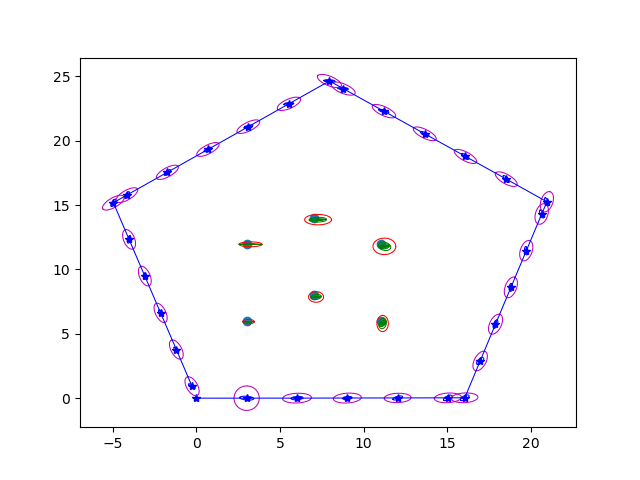
\includegraphics[width=0.95\textwidth]{EKF_SLAM_Result.png}
    \caption{EKF SLAM Result}
\end{figure}
\end{document}